\documentclass{cubeamer}
\usepackage[T1]{fontenc}
\usepackage[Q=yes]{examplep}

% Font stuff
\usepackage{fbb}
\setsansfont{Ubuntu}
\setmonofont{Inconsolata}
\setbeamerfont{footnote}{size=\tiny}
% \AtBeginDocument{\fontseries{sansserif}\selectfont}

\setbeamertemplate{itemize/enumerate body begin}{\small}
\setbeamertemplate{itemize/enumerate subbody begin}{\footnotesize}



\usepackage{hyperref}
\hypersetup{%
    colorlinks=true,
    linkcolor=gold,
    urlcolor=blue
}

\title{Introduction to \LaTeX}

\subtitle{%
Lecture 1
}

\author[Brian Keegan]{Professor Brian C. Keegan}
\date{\today} % or whatever the date you are presenting in is
\institute[Information Science]{Department of Information Science}
% \copyrightnotice{Published by the American Institute of Aeronautics and Astronautics, Inc., with permission}
\date{4 April 2023}

\begin{document}

\maketitle

% \cutoc

\section{Introductions}


\begin{frame}{Introductions}
    \begin{itemize}
        \item Name and pronouns
        \item Affiliations
        \item Reasons you are here
    \end{itemize}
\end{frame}

\begin{frame}{About me}
    \begin{itemize}
        \item Assistant Professor, Department of Information Science
        \item Computational social science, governing online commons, high-tempo online collaborations, cannabis informatics
        \item Didn't use \LaTeX{} until \textit{after} dissertation... a huge mistake!
        \item You are in version 2 of this course, feedback is very welcome!
        \item \href{mailto:brian.keegan@colorado.edu}{brian.keegan@colorado.edu}
    \end{itemize}
\end{frame}


\begin{frame}{Outline of lectures}
    \begin{itemize}
        \item Two lectures (April 4 \& 11) for two hours
        \item Lecture one
        \begin{itemize}
            \item Syntax, formatting, lists, tables, figures
        \end{itemize}
        \item Lecture two
        \begin{itemize}
            \item Math, document structure, bibliographies, presentations
        \end{itemize}
    \end{itemize}
\end{frame}

\begin{frame}{Resources}
    \begin{itemize}
        \item \href{https://www.latex-project.org/help/documentation/usrguide.pdf}{User Guide}. \textit{The \LaTeX{} Project}.
        \item \href{https://en.wikibooks.org/wiki/LaTeX}{\LaTeX}. \textit{Wikibooks}.
        \item \href{https://www.overleaf.com/learn}{Documentation}. \textit{Overleaf}.
        \item \href{https://www.learnlatex.org/en/}{Learn \LaTeX}.
        \item \href{https://www.andy-roberts.net/writing/latex}{Getting to Grips with \LaTeX}.
        \item \href{http://wch.github.io/latexsheet/latexsheet.pdf}{\LaTeXe~Cheat Sheet}.
        \item \href{https://tex.stackexchange.com/}{StackOverflow}.
    \end{itemize}
\end{frame}

\begin{frame}{What is \LaTeX?}
    \begin{itemize}
        \item \LaTeX{} is a markup language for typesetting documents
        \item It excels at math notation, multiple figures, \& large documents
        \item Not a WYSIWYG word processor like Microsoft Word, Google Docs, Apple Pages, Adobe InDesign, \textit{etc}.
        \item The code \textit{describing} your document's style and its content is compiled into a file
        \begin{itemize}
            \item Typically \href{https://en.wikipedia.org/wiki/PDF}{PDF} but \href{https://en.wikipedia.org/wiki/PostScript}{PostScript}, \href{https://en.wikipedia.org/wiki/Rich_Text_Format}{RTF}, \href{https://en.wikipedia.org/wiki/HTML}{HTML}, \href{https://en.wikipedia.org/wiki/Scalable_Vector_Graphics}{SVG} possible
            \item Converting from \LaTeX{} to Microsoft Word ``.doc'' is notoriously painful: \LaTeX{} $\rightarrow$ PDF $\rightarrow$ Adobe Acrobat $\rightarrow$ Microsoft Word
        \end{itemize}
    \end{itemize}
\end{frame}

\begin{frame}{History around \LaTeX}
    \begin{itemize}
        \item \href{https://en.wikipedia.org/wiki/Typography}{Typography} and \href{https://en.wikipedia.org/wiki/Typesetting}{typesetting} are art, technology, and professions originating in 10th-century China
        \item Early computers could not represent text \texttt{beyond simple monospaced Latin characters} like \href{https://en.wikipedia.org/wiki/Typewriter}{typewriters} or \href{https://en.wikipedia.org/wiki/Teleprinter}{teleprinters}
        \item \href{https://en.wikipedia.org/wiki/Donald_Knuth}{Donald Knuth} developed ``TeX'' in 1978 to support revisions to his famous book \href{https://en.wikipedia.org/wiki/The_Art_of_Computer_Programming}{\textit{The Art of Computer Programming}}
        \begin{itemize}
            \item Math formulae, non-Latin characters, multiple fonts
        \end{itemize}
        \item \LaTeX{} released in 1985 by Leslie Lamport with a focus on more user-friendly syntax and design patterns than TeX
    \end{itemize}
\end{frame}

\begin{frame}{Why use \LaTeX?}
    \centering
    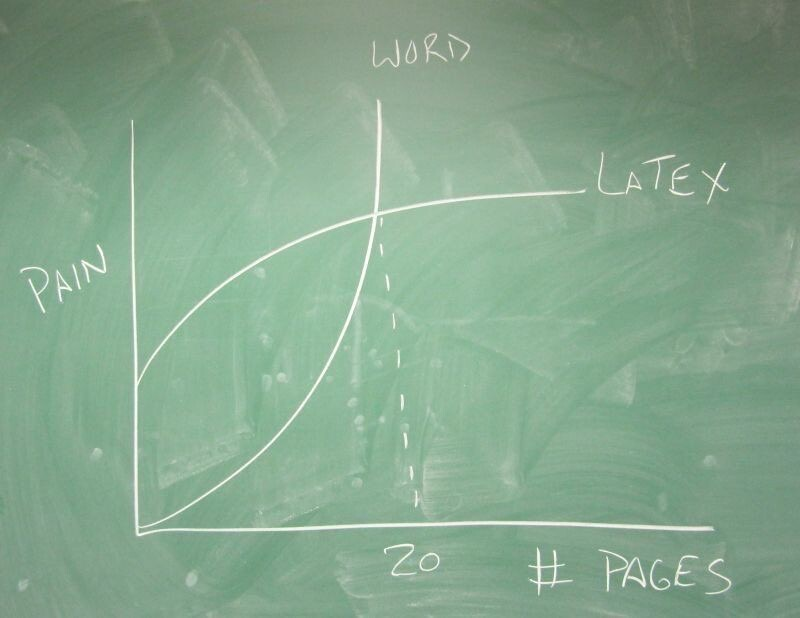
\includegraphics[width=.75\textwidth]{img/latex_vs_word.jpg}
    \footnote{\url{https://scholar.social/@caranha/110134212225485118}}
\end{frame}

\begin{frame}{Culture around \LaTeX}
    \begin{itemize}
        \item Common in math, physics, computer science, economics
        \item Mispronunciation is a classic out-group marker
        \begin{itemize}
            \item  LAH-tekh \textit{or} LAY-tekh; \textit{not} LAY-teks
        \end{itemize}
        \item \textbf{Costs}: learning and debugging technical syntax, configuring document structure and style
        \item \textbf{Benefits}: managing and customizing complex technical documents, professional-looking camera-ready output
        \begin{itemize}
            \item Manuscripts, theses, lecture notes, presentations
            \item These slides were written in \LaTeX!
        \end{itemize}
        \item Sharing, re-use, \& adaptation of \LaTeX{} code is common\footnote{Rotabi, R., Danescu-Niculescu-Mizil, C., \& Kleinberg, J. (2017a). \href{https://dl.acm.org/doi/abs/10.1145/3038912.3052652}{Competition and selection among conventions}; (2017b). \href{https://ojs.aaai.org/index.php/ICWSM/article/view/14870}{Tracing the Use of Practices Through Networks of Collaboration}.}
    \end{itemize}
\end{frame}

\begin{frame}{Development environment}
    \begin{itemize}
        \item \LaTeX{} can be run on your local machine
        \begin{itemize}
            \item \textit{Lots} of headaches around package management, fonts, \textit{etc}.
            \item \textbf{Windows} users should use \href{https://miktex.org/}{MikTeX}
            \item \textbf{Mac} users should use \href{https://www.tug.org/mactex/}{MacTex}
            \item Then use modern text editors/IDEs like \href{https://www.sublimetext.com/}{Sublime}, \href{https://atom.io/}{Atom}, \href{https://www.eclipse.org/ide/}{Eclipse}, \href{https://developer.apple.com/xcode/}{XCode}, \textit{etc.} to develop documents
        \end{itemize}
        \item We will use an online service called \href{https://www.overleaf.com}{Overleaf}
        \begin{itemize}
            \item The ``cloud'' handles package management, fonts, \textit{etc}.
            \item Free version is sufficient, \href{https://www.overleaf.com/user/subscription/plans}{paid} supports advanced features
            \item Misses some features of IDEs, but good for $>90\%$ of users
        \end{itemize}
    \end{itemize}
\end{frame}

\begin{frame}{Customizing and debugging}
    \begin{itemize}
        \item Customizing style of document through arcane commands and assembling a collection of libraries is the timesink
        \item Shifting mindset: Want to change the spacing for a bulleted list? 
        \begin{itemize}
            \item WYSIWYG: Highlight passage and apply desired formatting
            \item \LaTeX: Find variable, parameter, or operator or import a new library.
        \end{itemize}
        \item No one knows all of these moving parts and you are \textit{not} a ``bad'' user for consulting StackOverflow and documentation all the time!
        \begin{itemize}
            \item Many people have probably had a question like this before
            \item A \href{https://tex.stackexchange.com/a/300512/22575}{helpful answer} on StackOverflow
        \end{itemize}
        \item Changes may do nothing, break your whole build, or do something close to what you hoped $\rightarrow$ this is debugging!
    \end{itemize}
\end{frame}

% \begin{frame}{Computational thinking}
%     \begin{itemize}
%         \item Idiosyncratic syntax and archaic stack.
%         \item Debugging and iteration practices.
%         \item Abstracting, asking, and adapting resources.
%     \end{itemize}
% \end{frame}

\section{Syntax}

\begin{frame}[fragile]{Minimum viable example}
    \begin{itemize}
        \item This is the ``\href{https://en.wikipedia.org/wiki/\%22Hello,_World!\%22_program}{Hello World!}'' of \LaTeX
    \end{itemize}

    \begin{texcode}{Hello World!}
        \documentclass{article}
        \begin{document}
        Hello world!
        \end{document}
    \end{texcode}
    
    \begin{itemize}
        \item Also the most minimum example of a ``minimum viable example'' helpful for debugging the where/why/what of bugs
        \begin{itemize}
            \item a \verb|\documentclass| with type (``article'' is a common default)
            \item a ``document'' environment between a \verb|\begin| and \verb|\end|
        \end{itemize}
        \item All the content exists within the ``document'' environment
    \end{itemize}
\end{frame}

\begin{frame}[fragile]{Paragraphs, reserved characters, and comments}
    \begin{itemize}
        \item New paragraph created with an empty line
        \item There are some ``reserved'' characters with special meanings
        \begin{itemize}
            \item \verb|# $ % ^ & _ { } ~ \ | ...escape them with a backslash
            \item A \textit{very} common error, especially when copying from elsewhere
        \end{itemize}
        \item Comment lines with \verb|%|
    \end{itemize}
    
    \begin{texcode}{Paragraphs\, escaping reserved characters\, and comments}
        \documentclass{article}
        \begin{document}
        The apple costs \$2 \& the orange is \$1. % Paragraph 1
        
        Option \#2 has a 25\% chance of success. % Paragraph 2
        \end{document}
    \end{texcode}
\end{frame}

\begin{frame}[fragile]{Commands and environments}
    \begin{itemize}
        \item A command is invoked with a backslash and name of the command 
        \begin{itemize}
            \item Accepts arguments within curly braces \verb|{ }|
            \item Accepts optional parameters within square brackets \verb|[ ]|
        \end{itemize}
        \item An environment alters the behavior of larger parts of a document
        \begin{itemize}
            \item Exists between the \verb|\begin and \end| tags
        \end{itemize}
        \item Commands and environments can be nested
    \end{itemize}
    
    \begin{texcode}{Commands and environments}
        \documentclass{article}
        \begin{document}
        \begin{itemize} % Starts an itemize environment for a bulleted list
            \item I am \textbf{very} excited! % The \textbf{} command bolds the word very
        \end{itemize} % Stops the itemize environment
        \end{document}
    \end{texcode}
\end{frame}


\section{Front matter}

\begin{frame}[fragile]{Document environment}
    \begin{itemize}
        \item Always the first command because it defines layout and style
        \item There are \href{https://latex-tutorial.com/documentclass-latex/}{many document classes} available by default
        \begin{table}[]
            \centering
            \tiny
            \renewcommand{\arraystretch}{.8}
            \begin{tabular}{cl}
            \toprule
            \textbf{Class} & \textbf{Description} \\ \midrule
                \texttt{article} & Scientific manuscripts and reports \\
                \texttt{report} \& \texttt{book} & Documents with multiple chapters \\
                \texttt{letter} & Professional correspondence \\
                \texttt{minimal} & The most basic type used for debugging \\ \bottomrule
            \end{tabular}
        \end{table}
        \item More available at \href{http://www.latextemplates.com/}{LaTeX Templates}, \href{https://www.overleaf.com/gallery/}{Overleaf Gallery}, \textit{etc}.
        \begin{itemize}
            \item Many publishers have their own templates \& classes
        \end{itemize}
    \end{itemize}
    
    \begin{texcode}{Customizing document class}
        \documentclass[12pt,letter]{article} % Use 12-point font on a 8.5" x 11" letter paper
        \begin{document}
        Hello world!
        \end{document}
    \end{texcode}
    
\end{frame}


\begin{frame}[fragile]{Packages}
    \begin{itemize}
        \item Packages change and improve how default \LaTeX{} works
        \begin{itemize}
            \item Downloading and configuring packages locally will quickly make you want to use IDEs or cloud services offering package management
        \end{itemize}
        \item Import packages at top of the file, before \verb|\begin{document}|
        \item The \texttt{\href{https://ctan.org/pkg/geometry?lang=en}{geometry}} package customizes page layout
    \end{itemize}
    
    \begin{texcode}{Creating 2-inch margins}
        \documentclass{article}
        \usepackage[margin=2in]{geometry} % Import the geometry package and use 2-inch margins
        \begin{document}
        Hello world!
        \end{document}
    \end{texcode}
    
\end{frame}

\begin{frame}[fragile]{Preamble: Title and Author}
    \begin{itemize}
        \item You will likely also want a title and author
        \item Enter these into the ``preamble'' of the document before the content begins
        \begin{itemize}
            \item \verb|\title{}| formats and stores the name of the document
            \item \verb|\author{}| formats and stores the name(s) of the authors(s)
        \end{itemize}
    \end{itemize}
    
     \begin{texcode}{Adding a title and author}
        \documentclass{article}
        \begin{document}
        \title{The Document Title} % Store the name of the document
        \author{A Brilliant Writer} % Store the name of the author
        \maketitle % Make the title, including the author
        Hello world!
        \end{document}
    \end{texcode}
\end{frame}

\begin{frame}[fragile]{Preamble: Abstract and date}
    \begin{itemize}
        \item Including an abstract and date is also common
    \end{itemize}
    
     \begin{texcode}{Adding an abstract and title}
        \documentclass{article}
        \begin{document}
        \title{The Document Title}
        \author{A Brilliant Writer}
        \begin{abstract}
            A quick summary % Indenting within environments is helpful
        \end{abstract}
        \date{} % Leaving this empty defaults to today
        \maketitle
        Hello world!
        \end{document}
    \end{texcode}
\end{frame}

\section{Formatting}

\begin{frame}[fragile]{Sections: Basics}
    \begin{itemize}
        \item \LaTeX{} provides a few levels of sections (top to bottom):
        \begin{enumerate}
            \item \verb|\chapter| (specific to \texttt{book} and \texttt{report} classes)
            \item \verb|\section| (typically the top-level in an \texttt{article} manuscript)
            \item \verb|\subsection| 
            \item \verb|\subsubsection|
            \item \verb|\paragraph|
        \end{enumerate}
        \item The table of contents will reference these section names
    \end{itemize}
    
    \begin{texcode}{Adding a section}
        \documentclass{article}
        \begin{document}
        Hello world!
        \section{The next day} % Creates a new section
        It's still a beautiful day! % Content within new section
        \end{document}
    \end{texcode}
\end{frame}

\begin{frame}[fragile]{Sections: Formatting sections}
    \begin{itemize}
        \item Sections can formatted to have consistent styles, numbering, \textit{etc}.
        \item In the front matter, import the \texttt{\href{https://ctan.org/pkg/titlesec?lang=en}{titlesec}} package and invoke the \verb|\titleformat{}| command whose style you want to change
        \item Font, size, alignment, numbering, \textit{etc}. can be customized
    \end{itemize}
    \begin{center}
        \tiny
        \verb|\titleformat{⟨command⟩}[⟨shape⟩]{⟨format⟩}{⟨label⟩}{⟨sep⟩}{⟨before-code⟩}[⟨after-code⟩]|
    \end{center}
        
    \begin{texcode}{Changing section formatting}
        \documentclass{article}
        \usepackage{titlesec} % Imports the titlesec package
        % Update the \section definition to remove numbers, bold and large font, no indent
        \titleformat{\section}{\normalfont\Large\bfseries}{}{0pt}{}
        \begin{document}
        \section{Introduction}
        Hello world!
        \end{document}
    \end{texcode}
\end{frame}

\begin{frame}[fragile]{Text: Styling}
    \begin{itemize}
        \item Styles include: \textbf{bold}, \textit{italics}, \underline{underline}, \textsc{small caps}, and \texttt{typewriter}
        \item Can also use \textsubscript{textsubscript} and \textsuperscript{textsuperscript}
    \end{itemize}
    
    \begin{texcode}{Changing text style}
        \documentclass{article}
        \begin{document}
        \textbf{Hello world}, \textsc{what} a \textit{beautiful} \texttt{afternoon} on the 26\textsuperscript{th} day of July! 
        \end{document}
    \end{texcode}
\end{frame}

\begin{frame}[fragile]{Text: Size}
    \begin{itemize}
        \item Text can be {\tiny scaled} to {\huge several} pre-defined sizes
        \item List of \href{https://www.overleaf.com/learn/latex/Font_sizes\%2C_families\%2C_and_styles#Reference_guide}{font size names} and examples:
        \begin{itemize}
            \item \verb|\tiny|, \verb|\footnotesize|, \verb|\large|, \verb|\Huge|
        \end{itemize}
        \item Different style with command inside braces: \verb|{\size content}|
    \end{itemize}
    
    \begin{texcode}{Changing text size}
        \documentclass{article}
        \begin{document}
        {\tiny Hello world}, {\small what} a {\Large beautiful} day! 
        \end{document}
    \end{texcode}
\end{frame}

% TODO: Get different fonts and styles to show here
\begin{frame}[fragile]{Text: Font}
    \begin{itemize}
        \item There are hundreds of \href{https://tug.org/FontCatalogue/}{typefaces available} (\href{https://www.overleaf.com/learn/latex/Font_typefaces#Reference_guide}{Overleaf}), including \href{https://en.wikipedia.org/wiki/Times_New_Roman}{Times} and \href{https://en.wikipedia.org/wiki/Helvetica}{Helvetica}, but the default is \href{https://en.wikipedia.org/wiki/Computer_Modern}{Computer Modern}
        \begin{itemize}
            \item However, it's \href{https://tex.stackexchange.com/a/108746/22575}{non-trivial to change fonts} mid-document
        \end{itemize}
        \item Fonts have three coarse categories: serif, \textsf{sans serif}, and \texttt{monospaced}
        \item Change all the fonts in a document by importing font as a package
        \begin{itemize}
            \item ``\href{https://tug.org/FontCatalogue/fbb/}{fbb}'' (\href{https://en.wikipedia.org/wiki/Bembo}{Bembo}) is one of my favorite serif fonts with a fascinating history from the 15th century ...and what this presentation uses!
        \end{itemize}
    \end{itemize}
    
    \begin{texcode}{Changing font}
        \documentclass{article}
        \usepackage{fbb} % Change default font for whole document
        \begin{document}
        Hello world!
        \end{document}
    \end{texcode}
\end{frame}

\begin{frame}[fragile]{Text: Quote marks}
    \begin{itemize}
        \item \LaTeX{} has a very idiosyncratic syntax for formatting quote marks
        \begin{itemize}
            \item Probably the second most common bug newbies encounter!
        \end{itemize}
        \item Use the ``grave accent'' (tilde key to left of 1) for the left quote marks
        \item Use single or double quotes (to left of enter) for right quote marks
        \item Double quotes copied in from other documents may generate errors, unrecognizable characters, or just point wrong way
    \end{itemize}
    
    \begin{texcode}{Quote marks}
        \documentclass{article}
        \begin{document}
        A "quote" in a phrase. % Error or looks bad
        A ``quote'' in a phrase. % Canonical practice
        ``A `quote' in a phrase.'' % Quotes in quotes
        \end{document}
    \end{texcode}
    
\end{frame}

\begin{frame}[fragile]{Text: Diacritics and special characters}
    \begin{itemize}
        \item Encoding non-English characters is a famously hard problem
        \item \LaTeX{} designed on 128-character ASCII standard but can compose advanced characters with an \href{https://en.wikibooks.org/wiki/LaTeX/Special_Characters#Escaped_codes}{escaped code}
        \item Alternatively: declare the encoding with \texttt{\href{https://ctan.org/pkg/inputenc?lang=en}{inputenc}} package
        \item \href{https://en.wikibooks.org/wiki/LaTeX/Special_Characters#Other_symbols}{Other special characters} can still be used by escaping or commands
        \begin{itemize}
            \item \href{http://detexify.kirelabs.org/classify.html}{Detexify} is a super-cool tool!
        \end{itemize}
    \end{itemize}
    
    \begin{texcode}{Diacritics}
        \documentclass{article}
        \usepackage[utf8]{inputenc} % Tell LaTeX what encoding to use
        \begin{document}
        S\o{}ren Gonz\'{a}lez-Ag\"{u}ero % Use escaped ASCII characters to format
        Søren González-Agüero % Copy characters directly in if encoding declared
        \end{document}
    \end{texcode}
\end{frame}

\begin{frame}[fragile]{Content: Paragraph alignment and indents}
    \begin{itemize}
        % \item Another aesthetic or editorial option likely governed by a style class
        \item \verb|\indent| paragraphs that aren't, \verb|\noindent| that are
        \item Default paragraph alignment is fully justified on both sides
        \item Paragraphs can be aligned with commands or environments
    \end{itemize}
    
    \begin{table}[]
        \centering
        \tiny
        \renewcommand{\arraystretch}{.8}
        \begin{tabular}{lcc}
        \toprule
        \textbf{Alignment} & \textbf{Environment} & \textbf{Command} \\ \midrule
            Left justified & \texttt{flushleft} & \verb|\raggedright| \\
            Right justified & \texttt{flushright} & \verb|\raggedleft| \\
            Center & \texttt{center} & \verb|\centering| \\
            \bottomrule
        \end{tabular}
    \end{table}
    
    \begin{texcode}{Paragraph alignment}
        \documentclass{article}
        \begin{document}
        {\centering Centered in page}
        
        \noindent Don't indent me
        \end{document}
    \end{texcode}
\end{frame}

\begin{frame}[fragile]{Content: Line spacing}
    \begin{itemize}
        \item Non-default line spacing for aesthetic or editorial reasons?
        \begin{itemize}
            \item In practice, the class controls line spacing and don't mess with this
        \end{itemize}
        \item Use the \texttt{\href{https://ctan.org/pkg/setspace?lang=en}{setspace}} package
    \end{itemize}
    
    \begin{texcode}{Changing line spacing}
        \documentclass{article}
        \usepackage{setspace} % Imports the setspace package
        % \singlespacing % single spacing
        \onehalfspacing % one-half spacing
        % \setstretch{1.25} % 1.25 spacing
        \begin{document}
        \section{Introduction}
        Hello world!
        \end{document}
    \end{texcode}
\end{frame}

\section{Lists}

\begin{frame}[fragile]{Basics of lists}
    \begin{itemize}
        \item Lists are a common kinds of environment within \LaTeX
        \begin{itemize}
            \item \texttt{itemize} for bulleted lists
            \item \texttt{enumerate} for numbered lists
            \item \texttt{description} for qualitative lists
        \end{itemize}
        \item Lists can be nested up to a depth of four by default
    \end{itemize}
    
    \begin{texcode}{Lists}
        \documentclass{article}
        \begin{document}
        \begin{itemize} % An itemized list
            \item The first bulleted item
            \begin{enumerate} % Create a enumerate list beneath the itemize
                \item An indented numeric item % Still uses \item
            \end{enumerate} % Close the environment
            \item A second bulleted item % Add more items
        \end{itemize} % Close the environment
        \end{document}
    \end{texcode}
\end{frame}

\begin{frame}[fragile]{Helper packages}
    \begin{itemize}
        \item Use the \texttt{\href{https://ctan.org/pkg/enumitem?lang=en}{enumitem}} package to customize lists formats \& styles
        \begin{itemize}
            \item Spacing, margins, widths, indents, separation can all be customized
            \item \texttt{enumitem}'s ``noitemsep'' option makes lists single-spaced
        \end{itemize}
        \item If creating nested list environments is tiresome, try \texttt{\href{https://ctan.org/pkg/easylist?lang=en}{easylist}}!
    \end{itemize}
    
    \begin{texcode}{List helpers}
        \documentclass{article}
        \usepackage{enumitem}
        \begin{document}
        \begin{itemize}[noitemsep] % 
            \item The first bulleted item
            \item A second bulleted item
            \item A third bulleted item
        \end{itemize}
        \end{document}
    \end{texcode}
\end{frame}

\begin{frame}{Marionette me!}
    \begin{itemize}
        \item Let's make a non-trivial list together!
    \end{itemize}
\end{frame}

\section{Tables}

\begin{frame}[fragile]{Basics of tables}
    \begin{itemize}
        \item Tables in \LaTeX{} are powerful and frustrating
        \item Defaults requires using two environments
        \begin{itemize}
            \item \texttt{table} contains \texttt{tabular}, caption, and label
            \item \texttt{tabular} contains the content and markup describing the table
        \end{itemize}
        \item Reserved characters used extensively for tables
        \begin{itemize}
            \item \texttt{\&} column separator
            \item \texttt{\textbackslash\textbackslash} new row
        \end{itemize}
        \item There is a zen to creating \LaTeX{} tables by hand, but...
        \begin{itemize}
            \item \texttt{\href{https://pandas.pydata.org/docs/reference/api/pandas.DataFrame.to_latex.html}{.to\_latex()}} for pandas, \texttt{\href{https://cran.r-project.org/web/packages/stargazer/}{stargazer}} for R, \texttt{\href{http://www.ctan.org/tex-archive/support/excel2latex/}{excel2latex}} for Excel
            \item Web generators like \href{https://www.tablesgenerator.com/}{tablesgenerator.com} and \href{https://www.latex-tables.com/}{latex-tables.com}
        \end{itemize}
    \end{itemize}
\end{frame}

\begin{frame}[fragile]{A ``simple'' table}
        \begin{table} % Open the table environment
            \footnotesize
            \begin{tabular}{c|c} % Open the tabular environment
                label A & label B \\
                value 1 & value 2  \\
                value 3 & value 4
            \end{tabular}
            \caption{Caption} % Give a caption
            \label{tab:my_label} % Create a reference variable
        \end{table}
        
    \vspace{-2em}
    
    \begin{texcode}{A simple table}
        \documentclass{article}\begin{document}
        \begin{table} % Open the table environment
            \begin{tabular}{c|c} % Open the tabular environment
                label A & label B \\
                value 1 & value 2  \\
                value 3 & value 4
            \end{tabular}
            \caption{Caption} % Give a caption
            \label{tab:my_label} % Create a reference variable
        \end{table}
        \end{document}
    \end{texcode}
\end{frame}

\begin{frame}[fragile]{Intermediate tables}
    \begin{center}
        \verb|\begin{tabular}[pos]{table spec}|    
    \end{center}
    \begin{itemize}
        \item The \texttt{tablespec} is where the number, justification, and size of columns in the table are defined
        \begin{itemize}
            \item \texttt{l} for left, \texttt{c} for center, \texttt{r} for right, \texttt{p\{size\}} for text, \texttt{|} for lines
        \end{itemize}
        \item A \texttt{multicolumn} exists in the base package and often used with \texttt{\href{https://ctan.org/pkg/multirow?lang=en}{multirow}} package
        \item Common helper packages include \texttt{\href{https://ctan.org/pkg/array?lang=en}{array}} (advanced formatting), \texttt{\href{https://ctan.org/pkg/tabularx?lang=en}{tabularx}} (better text handling), \texttt{\href{https://ctan.org/pkg/booktabs?lang=en}{booktabs}} (prettier table elements), \texttt{\href{https://ctan.org/pkg/longtable?lang=en}{longtable}} (multi-page tables)
    \end{itemize}
\end{frame}

\begin{frame}{Marionette me!}
    \begin{itemize}
        \item Let's make a non-trivial table together!
    \end{itemize}
\end{frame}

\section{Figures}

\begin{frame}[fragile]{Basics of figures}
    \begin{itemize}
        \item \texttt{\href{https://ctan.org/pkg/graphicx?lang=en}{graphicx}} provides \verb|\includegraphics| that reads in image files
        \begin{itemize}
            \item Vector images (PDF, EPS, SVG) > raster images (JPEG, PNG, GIF)
            \item Scaling image size relative to document dimensions
        \end{itemize}
        \item Like tables, it often makes sense for the graphics to be embedded within a \texttt{figure} environment defining alignment, caption, and label
    \end{itemize}
    
    \begin{texcode}{A simple figure}
        \documentclass{article}
        \usepackage{graphicx}
        \begin{document}
        Some text.
        \begin{figure}
            \includegraphics[width=.5\textwidth]{image_file.png}
            \caption{Caption}
            \label{fig:my_label}
        \end{figure}
        \end{document}
    \end{texcode}
\end{frame}

\begin{frame}{Intermediate figures}
    \begin{itemize}
        \item You may want \href{https://www.overleaf.com/learn/latex/How_to_Write_a_Thesis_in_LaTeX_(Part_3)\%3A_Figures\%2C_Subfigures_and_Tables}{multiple sub-plots} in a single figure
        \begin{itemize}
            \item Use the \texttt{\href{https://ctan.org/pkg/caption?lang=en}{caption}} and \texttt{\href{https://ctan.org/pkg/subcaption?lang=en}{subcaption}} packages
        \end{itemize}
    \end{itemize}
\end{frame}

\begin{frame}[fragile]{Side-by-side sub-figures}
    \begin{texcode}{Side-by-side sub-figures}
        \documentclass{article}
        \usepackage{graphicx,subcaption}
        \begin{document}
        Some text.
        \begin{figure}
            \begin{subfigure}{.475\textwidth} % Subfigure width is a hair under half
                \includegraphics{image_file1.png}
                \caption{Caption for image 1}
                \label{fig:image1}
            \end{subfigure}\hfill
            \begin{subfigure}{.475\textwidth}
                \includegraphics{image_file2.png}
                \caption{Caption for image 2}
                \label{fig:image2}
            \end{subfigure}\caption{Caption for both images}
            \label{fig:both_images}
        \end{figure}
        \end{document}
    \end{texcode}
\end{frame}

\section{Next week}

\begin{frame}{Next week's topics}
    \begin{itemize}
        \item \textbf{Math}: symbols and equations
        \item \textbf{Modularity}: Multi-file documents
        \item \textbf{Bibliographies}: BibTeX and citations
        \item \textbf{Intermediate}: variables, counters, functions
        \item \textbf{Presentations}: \texttt{beamer}, \texttt{tikz}, and posters
        \item \textbf{Office Hours}: Debugging your projects!
    \end{itemize}
    
\end{frame}

\end{document}